%	The main skeletal structure
	\documentclass[crop,tikz,convert={outext=.svg,command=\unexpanded{/opt/homebrew/bin/pdf2svg \infile\space\outfile}},multi=false]{standalone}%	\documentclass[twocolumn]{report}
	\usepackage{setspace}
	\usepackage{graphicx}
		\DeclareGraphicsExtensions{.pdf,.png,.eps,.svg	ps}
	\usepackage{subcaption}
	\usepackage{lscape}
	\usepackage{pifont}
%	\usepackage{bbding}
	\usepackage{multirow}
	\usepackage{longtable}
	\usepackage[version=4]{mhchem}
	\usepackage{xfrac}
	\usepackage{color}
	\usepackage[colorlinks=true]{hyperref}
	\usepackage{gensymb}
	\usepackage{multicol}
		\setlength{\columnseprule}{0.4pt}
		\setlength{\columnsep}{5mm}
\makeatletter 
\newcounter{reaction} 
%%% >> for article << 
%\renewcommand\thereaction{C\,\arabic{reaction}} 
%%% << for article << 
%%% >> for report and book >> 
\renewcommand\thereaction{C\,\thechapter.\arabic{reaction}} 
\@addtoreset{reaction}{chapter} 
%%% << for report and book << 
\newcommand\reactiontag{\refstepcounter{reaction}\tag{\thereaction}} 
\newcommand\reaction@[2][]{\begin{equation}\ce{#2}% 
\ifx\@empty#1\@empty\else\label{#1}\fi% 
\reactiontag\end{equation}} 
\newcommand\reaction@nonumber[1]{\begin{equation*}\ce{#1}% 
\end{equation*}} 
\newcommand\reaction{\@ifstar{\reaction@nonumber}{\reaction@}} 
\makeatother 


	\usepackage[a4paper]{geometry}
	\usepackage{fullpage}
	\usepackage{fancyhdr}
%		\pagestyle{fancy}
%		\lhead{}
%		\chead{}
%		\rhead{\slshape \rightmark}
%		\fancyhead[LO,RE]{\slshape \leftmark} 
%		\fancyfoot[R]{\thepage} 
%	\renewcommand{\headrulewidth}{0.4pt} 
%	\renewcommand{\footrulewidth}{0.4pt} 
	\usepackage{cite}
	
%	\onehalfspacing
	\renewcommand{\baselinestretch}{1.5}
	
%	Footnote symbols
	\renewcommand{\thefootnote}{\fnsymbol{footnote}}

% Defining the chapter abstract area
%	\newenvironment{abstract}{\rightskip1in}{}

% Allow standard state notation
	\usepackage[varioref=false]{chemstyle}

% Allow for numbered examples
%	\usepackage{theorem,lipsum}
%	\theorembodyfont{\upshape}
%	\newtheorem{example}{Example}[chapter]
%	\newtheorem{question}{Question}[chapter]
%	\newtheorem{exercise}{Exercise}[chapter]
%	\newtheorem{concept}{Key Concept}[chapter]
%%%%%\begin{example}
%%%%%This is an example?
%%%%%\end{example}
%%%%%
%%%%%\begin{question}
%%%%%This is a quesiton?
%%%%%\end{question}

%%%%%FONT STUFF

%\usepackage[defaultfam,extralight,tabular,lining]{montserrat} %% Option 'defaultfam'
%%% only if the base font of the document is to be sans serif
%\usepackage[T1]{fontenc}
%\renewcommand*\oldstylenums[1]{{\fontfamily{Montserrat-TOsF}\selectfont #1}}

\usepackage{arev}
\usepackage[T1]{fontenc}
\usepackage{soul}

%%%%%TIKZ stuff
	\usepackage{tikz}
	\usepackage{pgfplots}
	\usetikzlibrary{decorations.pathmorphing,patterns,arrows,shapes.arrows}
	\usepgfplotslibrary{fillbetween}
	\tikzset{every picture/.style=remember picture}
		\newcommand{\mathnode}[1]{%
		\mathord{\tikz[baseline=(#1.base), inner sep = 0pt]{\node (#1) {$#1$};}}}

%%%%%% Grey stuff
%Need to define a shitload of greys...
\definecolor{gray1}{RGB}{240,240,240}
\definecolor{gray2}{RGB}{225,225,225}
\definecolor{gray3}{RGB}{210,210,210}
\definecolor{gray4}{RGB}{200,200,200}
\definecolor{gray5}{RGB}{180,180,180}


\begin{document}

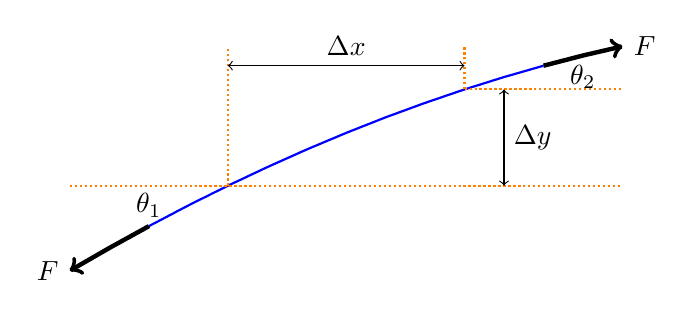
\begin{tikzpicture}[scale=1]
  \begin{axis}[
    grid=none,
%    xmax=10,
%    ymax=10, 
    axis x line=none,   
    width=10cm,
    height=5cm, 
    axis y line=none,
%    restrict y to domain=-1:9,
    enlargelimits,
    xlabel={$a$},
    xlabel style={ left},
    ylabel={$g(a)$},
    ylabel style={above },
    ticks=none,
%    ylabel near ticks,
%    xlabel near ticks,
    ]
  \addplot[blue,thick, domain=70:80,samples=100,] {sin(x)};% node[above]{$y=e^x$};
  \addplot[black,ultra thick, domain=80:82,samples=100,->] {sin(x)} node[right]{$F$};
  \addplot[black,ultra thick, domain=70:68,samples=100,->] {sin(x)} node[left]{$F$};
  \draw [ thick, densely dotted, draw=orange] (axis cs: 72,{sin(72)}) -- (axis cs: 72,({sin(82)});
  \draw [ thick, densely dotted, draw=orange] (axis cs: 68,{sin(72)}) -- (axis cs: 82,({sin(72)});
  \draw [ thick, densely dotted, draw=orange] (axis cs: 78,{sin(78)}) -- (axis cs: 78,({sin(82)});
  \draw [ thick, densely dotted, draw=orange] (axis cs: 78,{sin(78)}) -- (axis cs: 82,({sin(78)});
  \draw [ draw=black, <->] (axis cs:72 , {sin(80)}) -- node[above]{$\Delta x$} (axis cs:78 , {sin(80)} );
  \draw [ draw=black, <->] (axis cs:79 , {sin(72)}) -- node[right]{$\Delta y$} (axis cs:79 , {sin(78)} );
  \node at (axis cs: 81, {sin(79)}) {$\theta_2$} ;
  \node at (axis cs: 70, {sin(71)}) {$\theta_1$} ;
%  \addplot[mark=square*] coordinates {(1,6.8)};
%  \addplot[mark=square*] coordinates {(2,4.42)};
%  \addplot[mark=square*] coordinates {(3,3)};
%  \addplot[mark=square*] coordinates {(4,2.1)};
%  \addplot[mark=square*] coordinates {(5,1.4)};
%  \addplot[mark=square*] coordinates {(6,0.8)};
%  \addplot[mark=square*] coordinates {(7,0.55)};
\end{axis}
\end{tikzpicture}

\end{document}

% Use the following to include the graphics in the chapter
%
%
%\begin{figure}[htbp]
%\begin{center}
%\includegraphics[scale=1]{ch-x/images/filename.pdf}
%\caption[Caption for list of figures]{Full caption to appear beside the image}
%\label{fig:label}
%\end{center}
%\end{figure}
 